\subsubsection{1.1. Mô hình CNN baseline:}
\indent\indent Trước khi đi vào xây dựng mô hình MGAT + FastKAN/MLP, tôi tiến hành xây dựng và huấn luyện một kiến trúc CNN cơ sở (baseline) chỉ sử dụng dữ liệu hình ảnh. Mục tiêu của bước này là tạo ra một mốc hiệu năng tham chiếu (benchmark) để đánh giá sự cải thiện của các phương pháp đa phương thức sau này.\vspace{0.3cm}

\indent Kiến trúc của mô hình CNN baseline được minh họa tại \textbf{Hình \ref{fig:KTCNNBaseline}}, bao gồm các thành phần và cơ chế hoạt động như sau:
\begin{figure}[H]
    \centering
    \scalebox{0.6}{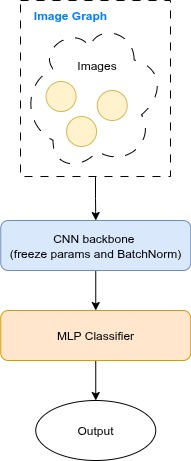
\includegraphics{images/part-02/chap-02/sec-01/CNNBaseline.jpg}}
    \vspace{0.3cm}
    \caption{Kiến trúc của mô hình CNN baseline}
    \label{fig:KTCNNBaseline}
\end{figure}

\textbf{Đầu vào (Image Graph):} Đây là dữ liệu ảnh đã được tiền xử lý bằng cách dùng các transforms từ các CNN backbone tương ứng.\vspace{0.3cm}

\textbf{Đầu ra (Output):} Kết quả dự đoán xác suất cho từng hình ảnh, sau đó tiền hành lấy trung bình cộng xác suất lại và cho ra kết quả phân lớp cuối cùng trên một mẫu đồ thị.\vspace{0.3cm}

\newpage
\textbf{Quy trình xử lý:}\vspace{-0.1cm}
\begin{itemize}[label={--}, itemsep=3pt]    
    \item \textbf{Trích xuất đặc trưng:} Tôi sử dụng 6 kiến trúc CNN bao gồm \textbf{ResNet18}, \textbf{RegNetX400MF}, \textbf{MobileNetV3 Large}, \textbf{MobileNetV3 Small}, \textbf{DenseNet121} và \textbf{ShuffleNetV2 1.0x} đã được huấn luyện trước trên tập dữ liệu khổng lồ ImageNet. Điểm quan trọng trong thiết kế này là cơ chế "đóng băng" (freezing):
    \begin{itemize}[label={+}]
        \item \textbf{Freeze Parameters:} Toàn bộ trọng số và bias của các lớp tích chập được giữ nguyên, không cập nhật trong quá trình lan truyền ngược. Điều này giúp bảo toàn khả năng nhận diện các đặc trưng cơ bản (cạnh, góc, textur) mà mạng đã học được từ ImageNet.
        \item \textbf{Freeze BatchNorm:} Các lớp Batch Normalization cũng được chuyển sang chế độ đánh giá (\textit{eval mode}), nghĩa là chúng sử dụng các giá trị trung bình (mean) và phương sai (variance) toàn cục đã học trước đó thay vì tính toán lại trên từng batch dữ liệu huấn luyện mới. Điều này đảm bảo tính ổn định của đặc trưng đầu ra.
    \end{itemize}
    
    \item \textbf{Bộ phân lớp (MLP Classifier):}  Các đặc trưng sau khi đi qua Backbone sẽ được đưa vào một mạng MLP. Đây là thành phần duy nhất có thể học được. Nhiệm vụ của MLP là học cách ánh xạ từ không gian đặc trưng của ImageNet sang không gian nhãn của ICH.
\end{itemize}